% LuaLaTeX文書; 文字コードはUTF-8
\documentclass[unicode,12pt]{beamer}% 'unicode'が必要
\usepackage{luatexja}% 日本語したい
\usepackage[ipaex]{luatexja-preset}% IPAexフォントしたい
\renewcommand{\kanjifamilydefault}{\gtdefault}% 既定をゴシック体に

\usepackage{amssymb,amsmath,ascmac}
\usepackage{derivative}

\usepackage{multirow}
\usepackage{bm}

\graphicspath{{../fig/}}

\usepackage{booktabs}
\usepackage{tikz}
\usepackage{xparse}
\usetikzlibrary{shapes,arrows}
%% define fancy arrow. \tikzfancyarrow[<option>]{<text>}. ex: \tikzfancyarrow[fill=red!5]{hoge}
\tikzset{arrowstyle/.style n args={2}{inner ysep=0.1ex, inner xsep=0.5em, minimum height=2em, draw=#2, fill=black!20, font=\sffamily\bfseries, single arrow, single arrow head extend=0.4em, #1,}}
\NewDocumentCommand{\tikzfancyarrow}{O{fill=black!20} O{none}  m}{
\tikz[baseline=-0.5ex]\node [arrowstyle={#1}{#2}] {#3 \mathstrut};}

%目次スライド
\AtBeginSection[]{
  \frame{\tableofcontents[currentsection]}
}
%アペンディックスのページ番号除去
\newcommand{\backupbegin}{
\newcounter{framenumberappendix}
\setcounter{framenumberappendix}{\value{framenumber}}
}
\newcommand{\backupend}{
\addtocounter{framenumberappendix}{-\value{framenumber}}
\addtocounter{framenumber}{\value{framenumberappendix}} 
}

%%%%%%%%%%%  theme  %%%%%%%%%%%
\usetheme{Copenhagen}
% \usetheme{Metropolis}
% \usetheme{CambridgeUS}
% \usetheme{Berlin}

%%%%%%%%%%%  inner theme  %%%%%%%%%%%
% \useinnertheme{default}

% %%%%%%%%%%%  outer theme  %%%%%%%%%%%
\useoutertheme{default}
% \useoutertheme{infolines}

%%%%%%%%%%%  color theme  %%%%%%%%%%%
%\usecolortheme{structure}

%%%%%%%%%%%  font theme  %%%%%%%%%%%
\usefonttheme{professionalfonts}
%\usefonttheme{default}

%%%%%%%%%%%  degree of transparency  %%%%%%%%%%%
%\setbeamercovered{transparent=30}

% \setbeamertemplate{items}[default]

%%%%%%%%%%%  numbering  %%%%%%%%%%%
% \setbeamertemplate{numbered}
\setbeamertemplate{navigation symbols}{}
\setbeamertemplate{footline}[frame number]

\title{粘着剤の基礎知識と評価法}
\subtitle{~ 第六章 タッキファイヤーの働きについて ~}
\author[SDL Inc. 佐々木]{佐々木 裕\thanks{hsasaki@softmatters.net}}
\institute[]{元 東亞合成株式会社\\ソフトマターデザインラボ合同会社}
\date{2024/6/24}

\begin{document}

%%%%%
% 1 P
%%%%%
\maketitle

\begin{frame} 
    \tableofcontents[]
\end{frame} 


\section{タッキファイヤーとは?}
\subsection{一般的なタッキファイヤーの説明}

\begin{frame}
	\frametitle{タッキファイヤーとは}
		\begin{itemize}
			\item タッキファイヤーとは
			\begin{itemize}
				\item 粘着剤のベースとなるポリマーに添加することにより、粘着特性を改良できる添加剤
				\item 主としてタック(瞬間的なベタつき)を付与することが名前の由来。
			\end{itemize}
			\item 一般的な特徴
			\begin{itemize}
				\item \alert{分子量が数千程度}の無定形オリゴマー
				\item 一般的に\alert{高い軟化点}を有し、室温で固体
				\item 幅広いベースポリマーと\alert{相溶}
			\end{itemize}
		\end{itemize}
\end{frame}

\subsection{タッキファイヤーの種類と構造}
\begin{frame}
	\frametitle{タッキファイヤーの種類}
		\begin{itemize}
			\item 一般のテキストでは、以下のようにまとめられている。
			\item 大きく分類すれば、天然系と合成系
		\end{itemize}
	\begin{table}[tb]
		\scriptsize
		\centering
			\begin{tabular}{ccl}
				\toprule
				\multirow{4}{*}{天然樹脂系}	&\multirow{2}{*}{ロジン系}&ロジン \\
											&	&ロジン誘導体(水素化、エステル化等) \\
											\cmidrule(lr){2-3}
											&\multirow{2}{*}{テルペン系}& テルペン樹脂、テルペンフェノール樹脂\\ 
											& & 水素化テルペン樹脂 \\
				\midrule
				\multirow{4}{*}{合成樹脂系} &\multirow{2}{*}{石油樹脂系}& 脂肪族系、芳香族系、共重合系 \\ 
											&	& 水素化石油樹脂 \\
											\cmidrule(lr){2-3}
											&\multirow{2}{*}{その他}& フェノール樹脂、キシレン樹脂 \\
											&	&インデン樹脂、ケトン樹脂\\ 
				\bottomrule
			\end{tabular}
	\end{table}
\end{frame}

\begin{frame}
	\frametitle{ロジン誘導体}
		\begin{columns}[c, onlytextwidth]
			\column{.55\linewidth}
				\begin{itemize}
					\item 主として松ヤニから製造
					\item アビエチン酸を主成分
					\item 淡黄色から褐色の固体
					\item 多様な樹脂に相溶する
					\item エステル誘導体が主
					\item 二重結合が酸化されやすい
					\begin{itemize}
						\item 不均化、水添で改質
					\end{itemize}
					\item 耐熱性向上
					\begin{itemize}
						\item 二量化
						\item マレイン酸等の付加
					\end{itemize}
				\end{itemize}
			\column{.45\linewidth}
				\centering
				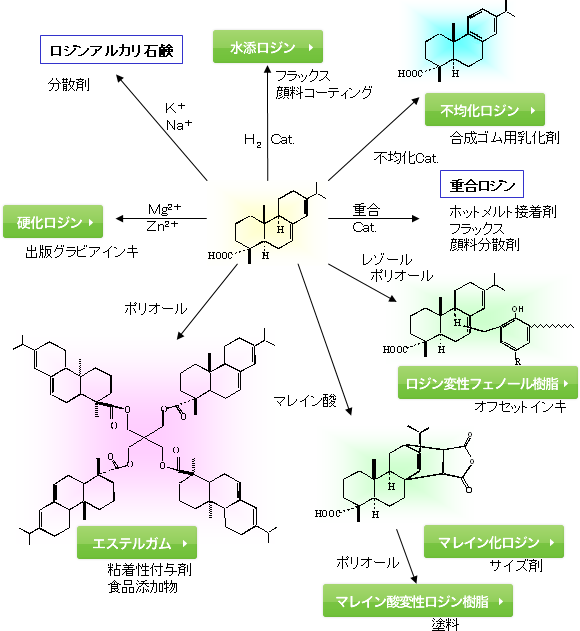
\includegraphics[width=\textwidth]{tackifier_rosin.png}

				\href{https://www.arakawachem.co.jp/jp/technology/catalog/02.html}{「荒川化学」のサイト}
		\end{columns}

\end{frame}
\begin{frame}
	\frametitle{テルペン系}
		\begin{itemize}
			\item イソプレンユニット(C5)を基本単位とする天然素材
			\item 各種誘導体が多様な用途に用いられている。
		\end{itemize}
		\centering
			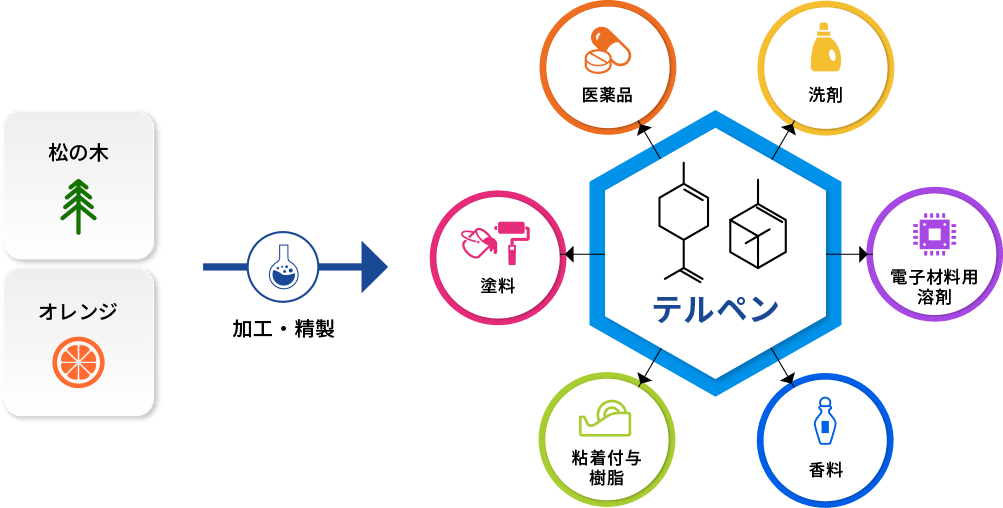
\includegraphics[width=\textwidth]{tackifier_terpene.png}

		\href{https://www.nipponterpene.co.jp/about/}{「日本テルペン化学」のサイト}
\end{frame}

\begin{frame}
	\frametitle{石油樹脂の例}
	\begin{itemize}
		\item 原油からの C5 留分と C9 留分を原料とする石油樹脂
		\item 成分比の制御により特性を調整
		\item 東ソーのペトロタックを例示
		\item Mw = 1000 to 4000 のオリゴマー
	\end{itemize}
	
		\centering
			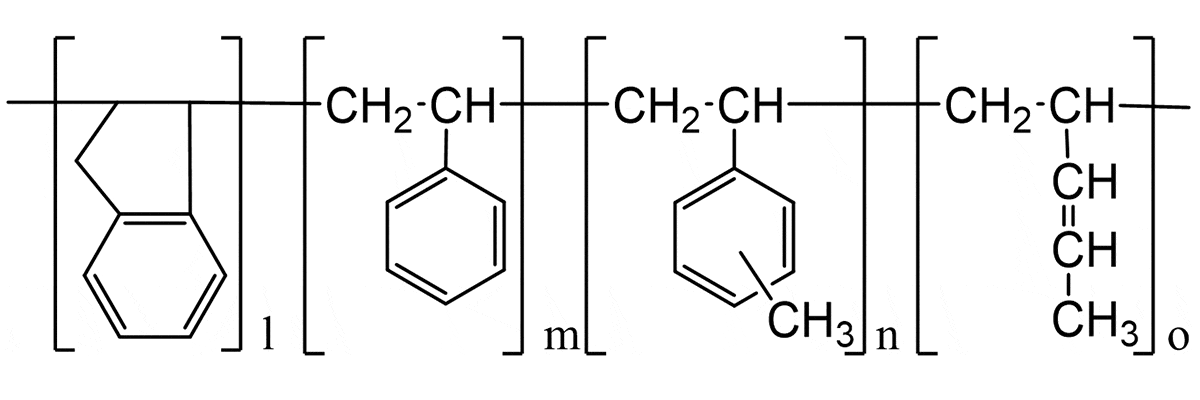
\includegraphics[width=\textwidth]{tackifier_petroleun_polymer.png}
	
			\href{https://www.tosoh.co.jp/product/polymer/c5_c9_type_petroleun_polymer_resins.html}{「東ソー」のサイト}
\end{frame}

\subsection{タッキファイヤーの相溶性}
\begin{frame}
	\frametitle{粘着剤の分類と特徴}

		主要な粘着剤の分類と特徴を以下にまとめた

		\begin{table}[tb]
			\tiny
			\centering
				\begin{tabular}{ccl}
				\toprule
				分類&エラストマー&特徴 \\
				\midrule
				\multirow{4}{*}{ゴム系}&\multirow{4}{*}{天然ゴム}&天然ゴムは価格が安い\\
				&&\textcolor{blue}{被着体の選択性が小さい}\\
				&&\textcolor{blue}{極性基を有していないので粘着力の上昇が小さい}\\
				&&耐熱、耐候性に劣る\\
				\midrule
				\multirow{4}{*}{アクリル系}&\multirow{4}{*}{アクリル酸エステル共重合体}&\alert{ポリマー自体で粘着性がある}\\
				&&\alert{変性が自由}\\
				&&ゴム系に比べ耐熱、耐候性に優れる\\
				&&被着体の選択性がある\\
				\midrule
				\multirow{4}{*}{シリコーン系}&\multirow{4}{*}{シリコーンゴム}&適用温度範囲が広い\\
				&&耐熱、耐寒性に優れる\\
				&&耐薬品性、耐候性に優れる\\
				&&\textcolor{blue}{価格が高い}\\
				\midrule
				\multirow{4}{*}{ウレタン系}&\multirow{4}{*}{ウレタン樹脂}&再はく離性に優れる\\
				&&低臭気、低皮膚刺激性に優れる\\
				&&透湿性に優れる\\
				&&\textcolor{blue}{強粘着性、タックがでにくい}\\
				\bottomrule
				\end{tabular}
		\end{table}
\end{frame}

\begin{frame}
	\frametitle{タッキファイヤーの相溶性}
		\begin{itemize}
			\item 相溶性は溶解度パラメタで理解可能(第三章)
			\item 似たものは似たものに溶ける
		\end{itemize}

			\vspace{3mm}
			\centering
				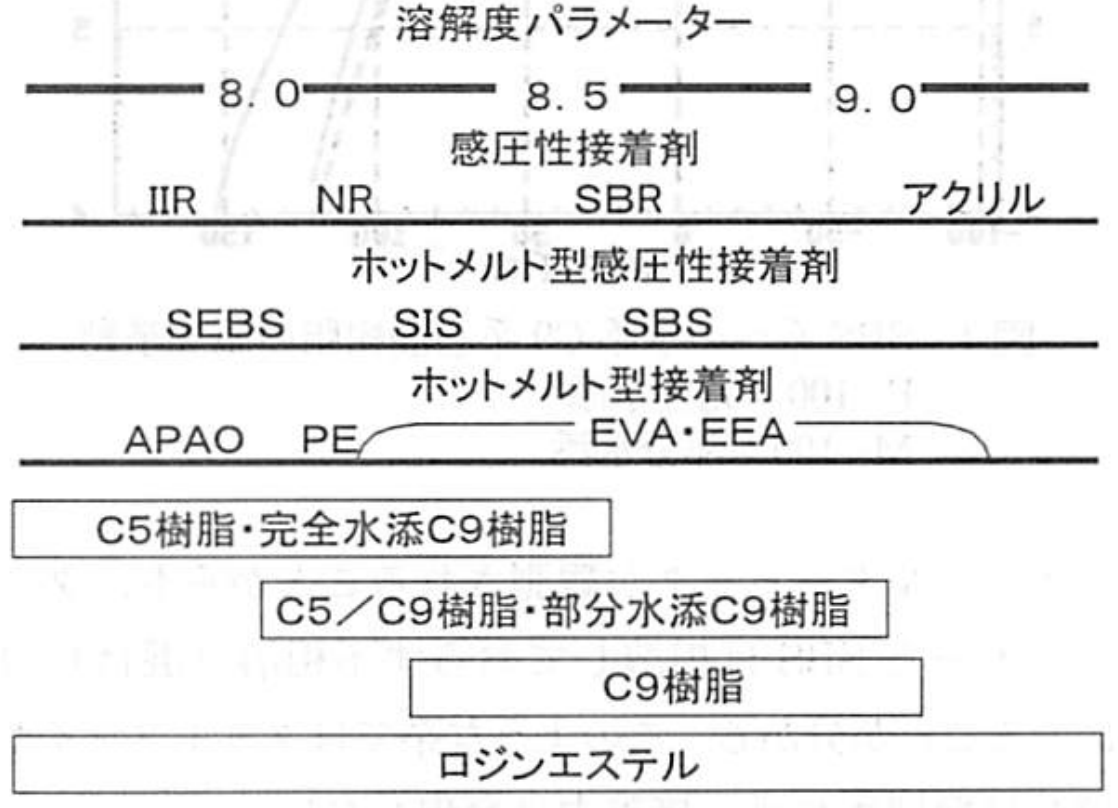
\includegraphics[width=.6\textwidth]{souyousei.png}
\end{frame}

\begin{frame}
	\frametitle{「タッキファイヤーとは」のまとめ}
        \begin{boxnote}
            \vspace{-3mm}
            \begin{itemize}
                \item 一般的なタッキファイヤーの説明
                    \begin{itemize}
                        \item ベースポリマーに添加することで粘着特性(とくにタック)を改良
                        \begin{itemize}
							\item \alert{分子量が数千程度}の無定形オリゴマー
							\item 一般的に\alert{高い軟化点}を有し、室温で固体
							\item 幅広いベースポリマーと\alert{相溶}
						\end{itemize}
                    \end{itemize} 
                \item タッキファイヤーの種類と構造
                    \begin{itemize}
                        \item 天然樹脂系(ロジン誘導体、テルペン系等)
                        \item 合成系(石油樹脂等)
                    \end{itemize} 
                \item タッキファイヤーの相溶性
                    \begin{itemize}
                        \item SP値が近いものが相溶する
						\item 分子量が低いことも幅広い相溶性に有効
                    \end{itemize}
            \end{itemize}
        \end{boxnote}
\end{frame}

\section{粘着特性に対する経験則}
\subsection{Dahlquist のクライテリア}
\setcounter{footnote}{0}
\begin{frame}
	\frametitle{Dahlquist のクライテリアとは?}
		% \begin{block}{Dahlquist のクライテリアとは?}
			\begin{itemize}
				\item 粘着性(タック)発現に関する基本的な経験則
				\item 1969 年に Dahlquist がその著書\footnote{Dahlquist,C.A., "Adhesion,Fundamental \& Practice", McLaren \& Sons, Ltd, London (1969)}で提唱
				\item タックを発現するためには、\\\alert{粘着剤の貯蔵弾性率 $G^{\prime} \leq$ 0.1 MPa }
			\end{itemize}

			\begin{columns}[c, onlytextwidth]
				\column{.4\linewidth}
						\centering
							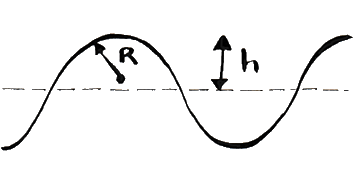
\includegraphics[width=\textwidth]{Dahlquist.png}
				\column{.6\linewidth}
					\begin{itemize}
						\item 左図のような表面凸凹を想定
						\item これと接触できる弾性率を\\以下の式で概算
					\end{itemize}

					\vspace{-6mm}
					\begin{align*}
						G_c = W \cdot \sqrt{\dfrac{R}{h^3}}
					\end{align*}
			\end{columns}
\end{frame}


\subsection{Chang の窓}
\begin{frame}
	\frametitle{弾性率と時間}
		\begin{itemize}
			\item 時間の概念を周波数として導入
			\begin{itemize}
				\item タックを発現する時間を $f=10^2 \Leftrightarrow 10^{-2} sec$
				\item 保持する時間を $f=10^{-2} \Leftrightarrow 10^{2} sec$
			\end{itemize}
		\end{itemize}
		\centering
			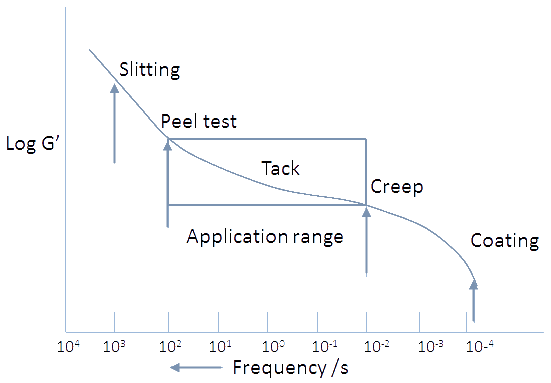
\includegraphics[width=.6\textwidth]{ChangFrequencies_1.png}

		\href{https://www.stevenabbott.co.uk/practical-adhesion/chang.php}{このグラフのサイト}
\end{frame}

\begin{frame}
	\frametitle{Chang の窓}
		\begin{itemize}
			\item さらに、エネルギー散逸を表す損失弾性率も導入
			\item 周波数の窓の中に、貯蔵および損失弾性率の値を\\プロット
			\begin{itemize}
				\item 高い周波数(100/sec)
				\item 低い周波数(0.01/sec)
			\end{itemize}
			\item 粘着剤の振る舞いを4つの領域に分類
		\end{itemize}

		\vspace{3mm}
		\centering
			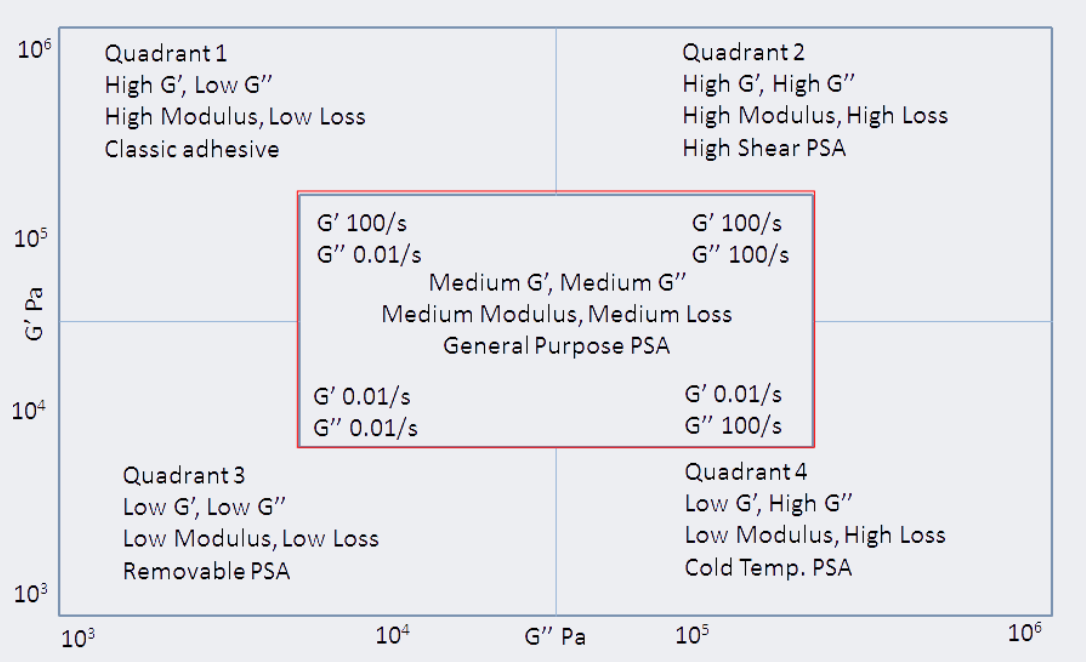
\includegraphics[width=.5\textwidth]{ChangFrequencies_2.png}

			\href{https://www.stevenabbott.co.uk/practical-adhesion/chang.php}{このグラフのサイト}
\end{frame}

\subsection{「Chang の窓」の意味するものは?}
\begin{frame}
	\frametitle{「Chang の窓」のポイント}
	\begin{alertblock}{損失弾性率 $G^{\prime \prime}$ の振る舞いが重要}
		\begin{itemize}
			\item 高い周波数(100/sec)
			\begin{itemize}
				\item 高い $G^{\prime \prime} \Leftrightarrow$ 高い流動性:クイックタッキネス
			\end{itemize}
			\item 低い周波数(0.01/sec)
			\begin{itemize}
				\item 低い $G^{\prime \prime} \Leftrightarrow$ 変形を抑止;保持力向上
			\end{itemize}
		\end{itemize}

		\vspace{3mm}
		\centering
			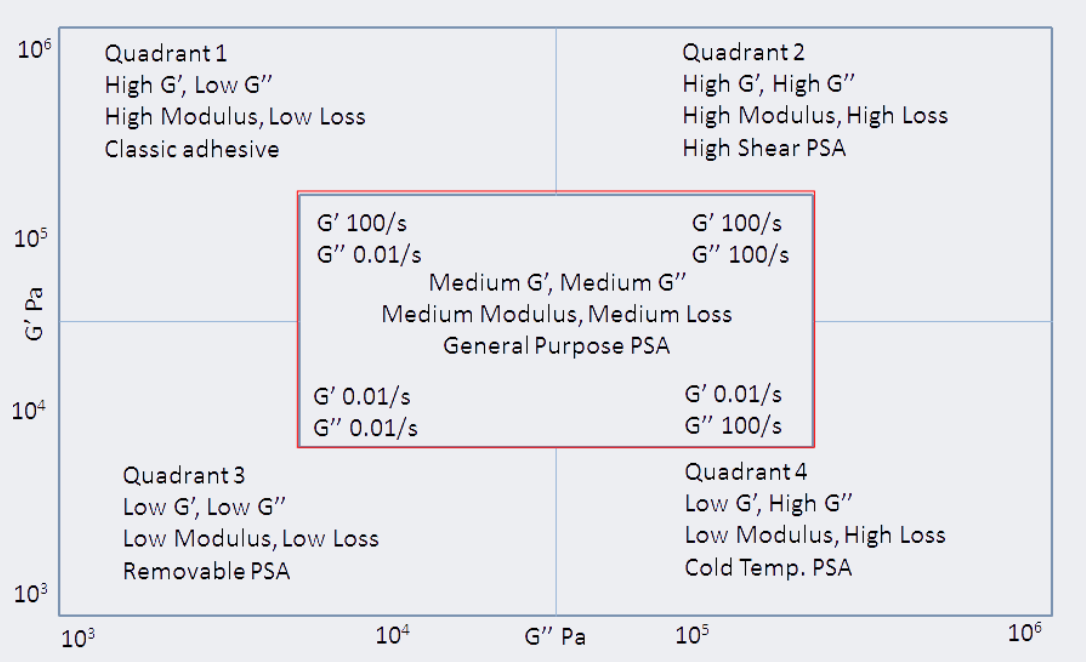
\includegraphics[width=.5\textwidth]{ChangFrequencies_2.png}
	\end{alertblock}	
\end{frame}

\begin{frame}
	\frametitle{「Chang の窓」のポイント}
	\begin{exampleblock}{それぞれの領域の意味}
		\begin{itemize}
			\item Quadrant 1: $G^{\prime \prime}$ が低いためタックが弱い
			\item Quadrant 2: $G^{\prime}, G^{\prime \prime}$ が高くタックもあり保持力もある
			\item Quadrant 3: $G^{\prime}, G^{\prime \prime}$ ともに低いので再剥離が容易
			\item Quadrant 4: $G^{\prime}$ が低いので凝集破壊しやすい
		\end{itemize}

		\vspace{3mm}
		\centering
			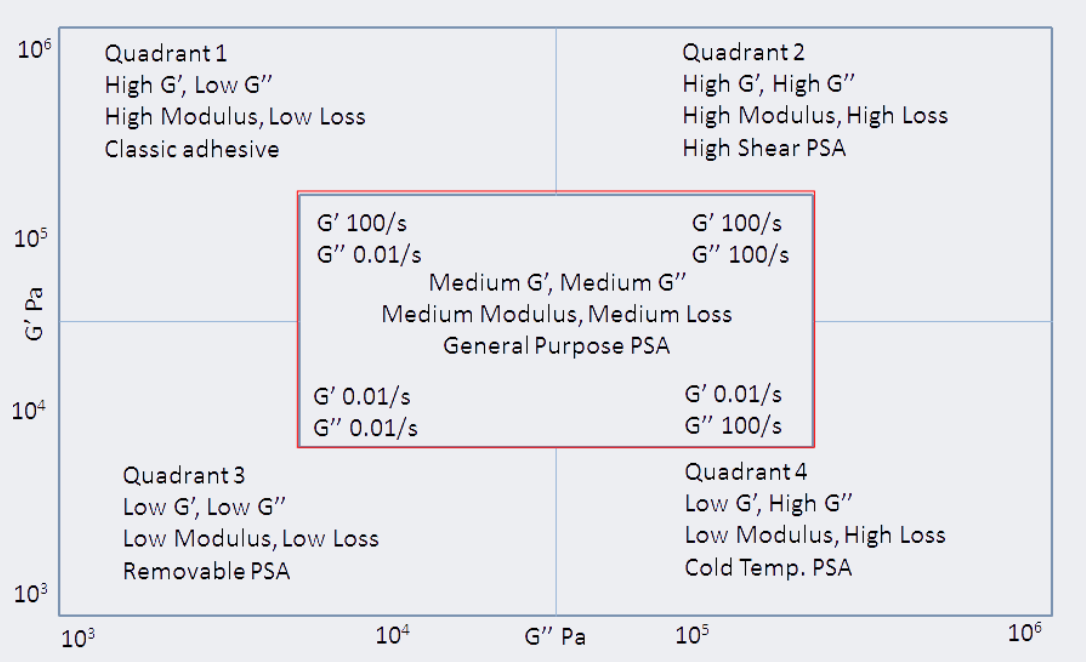
\includegraphics[width=.4\textwidth]{ChangFrequencies_2.png}

			\large
			\alert{「結局、$G^{\prime}, G^{\prime \prime}$ のバランスが重要!」}
	\end{exampleblock}	
\end{frame}

\begin{frame}
	\frametitle{「粘着特性に対する経験則」のまとめ}
        \begin{boxnote}
            \vspace{-3mm}
            \begin{itemize}
                \item Dahlquist のクライテリア
                    \begin{itemize}
                        \item 基材の表面凸凹に対応するための最大限の $G'$ を定義
                        \item 粘着剤の貯蔵弾性率 $G' < 0.1$ MPa
                    \end{itemize} 
                \item Chang の窓
                    \begin{itemize}
                        \item 各種挙動に対応する時間の概念を周波数として導入
                        \item それぞれの周波数での貯蔵、損失弾性率を定義
                    \end{itemize} 
                \item 「Chang の窓」の意味
                    \begin{itemize}
                        \item 「結局、$G', G''$ のバランスが重要!」
                    \end{itemize}
            \end{itemize}
        \end{boxnote}
\end{frame}

\section{タッキファイヤーの添加効果}

\subsection{各種エラストマーとタッキファイヤー}
\begin{frame}
	\frametitle{タッキファイヤーの添加}
	\begin{itemize}
		\item 各種エラストマーとの相溶性
		\begin{itemize}
			\item 相溶性は溶解度パラメタで理解可能(第三章)
			\item 似たものは似たものに溶ける
			\item \alert{分子量が数千程度}の無定形オリゴマー
		\end{itemize}
	\end{itemize}
	\vspace{3mm}
				\centering
					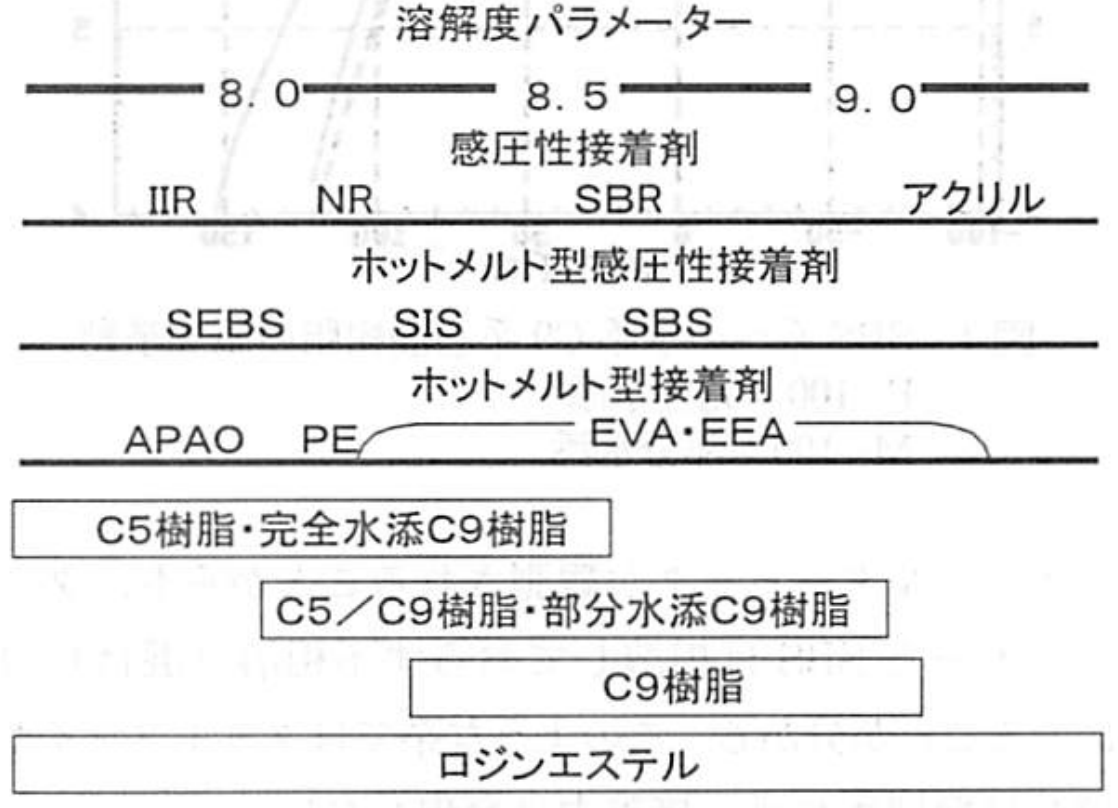
\includegraphics[width=.6\textwidth]{souyousei.png}
\end{frame}

\subsection{タック発現の機構}
\begin{frame}
	\frametitle{ゴム系ベースポリマーがタックが低い理由}
		\begin{block}{ゴム状エラストマー単独の粘弾性特性}
		\begin{itemize}
			\item ガラス転移温度が低い(-60 to -40 ℃)
			\item ラバープラトーの貯蔵弾性率が比較的に高い
			\begin{itemize}
				\item 絡みやすいため $M_E$ が小さい
				\item 貯蔵弾性率が反比例して大きい
			\end{itemize}
		\end{itemize}
	\end{block}
		\centering
			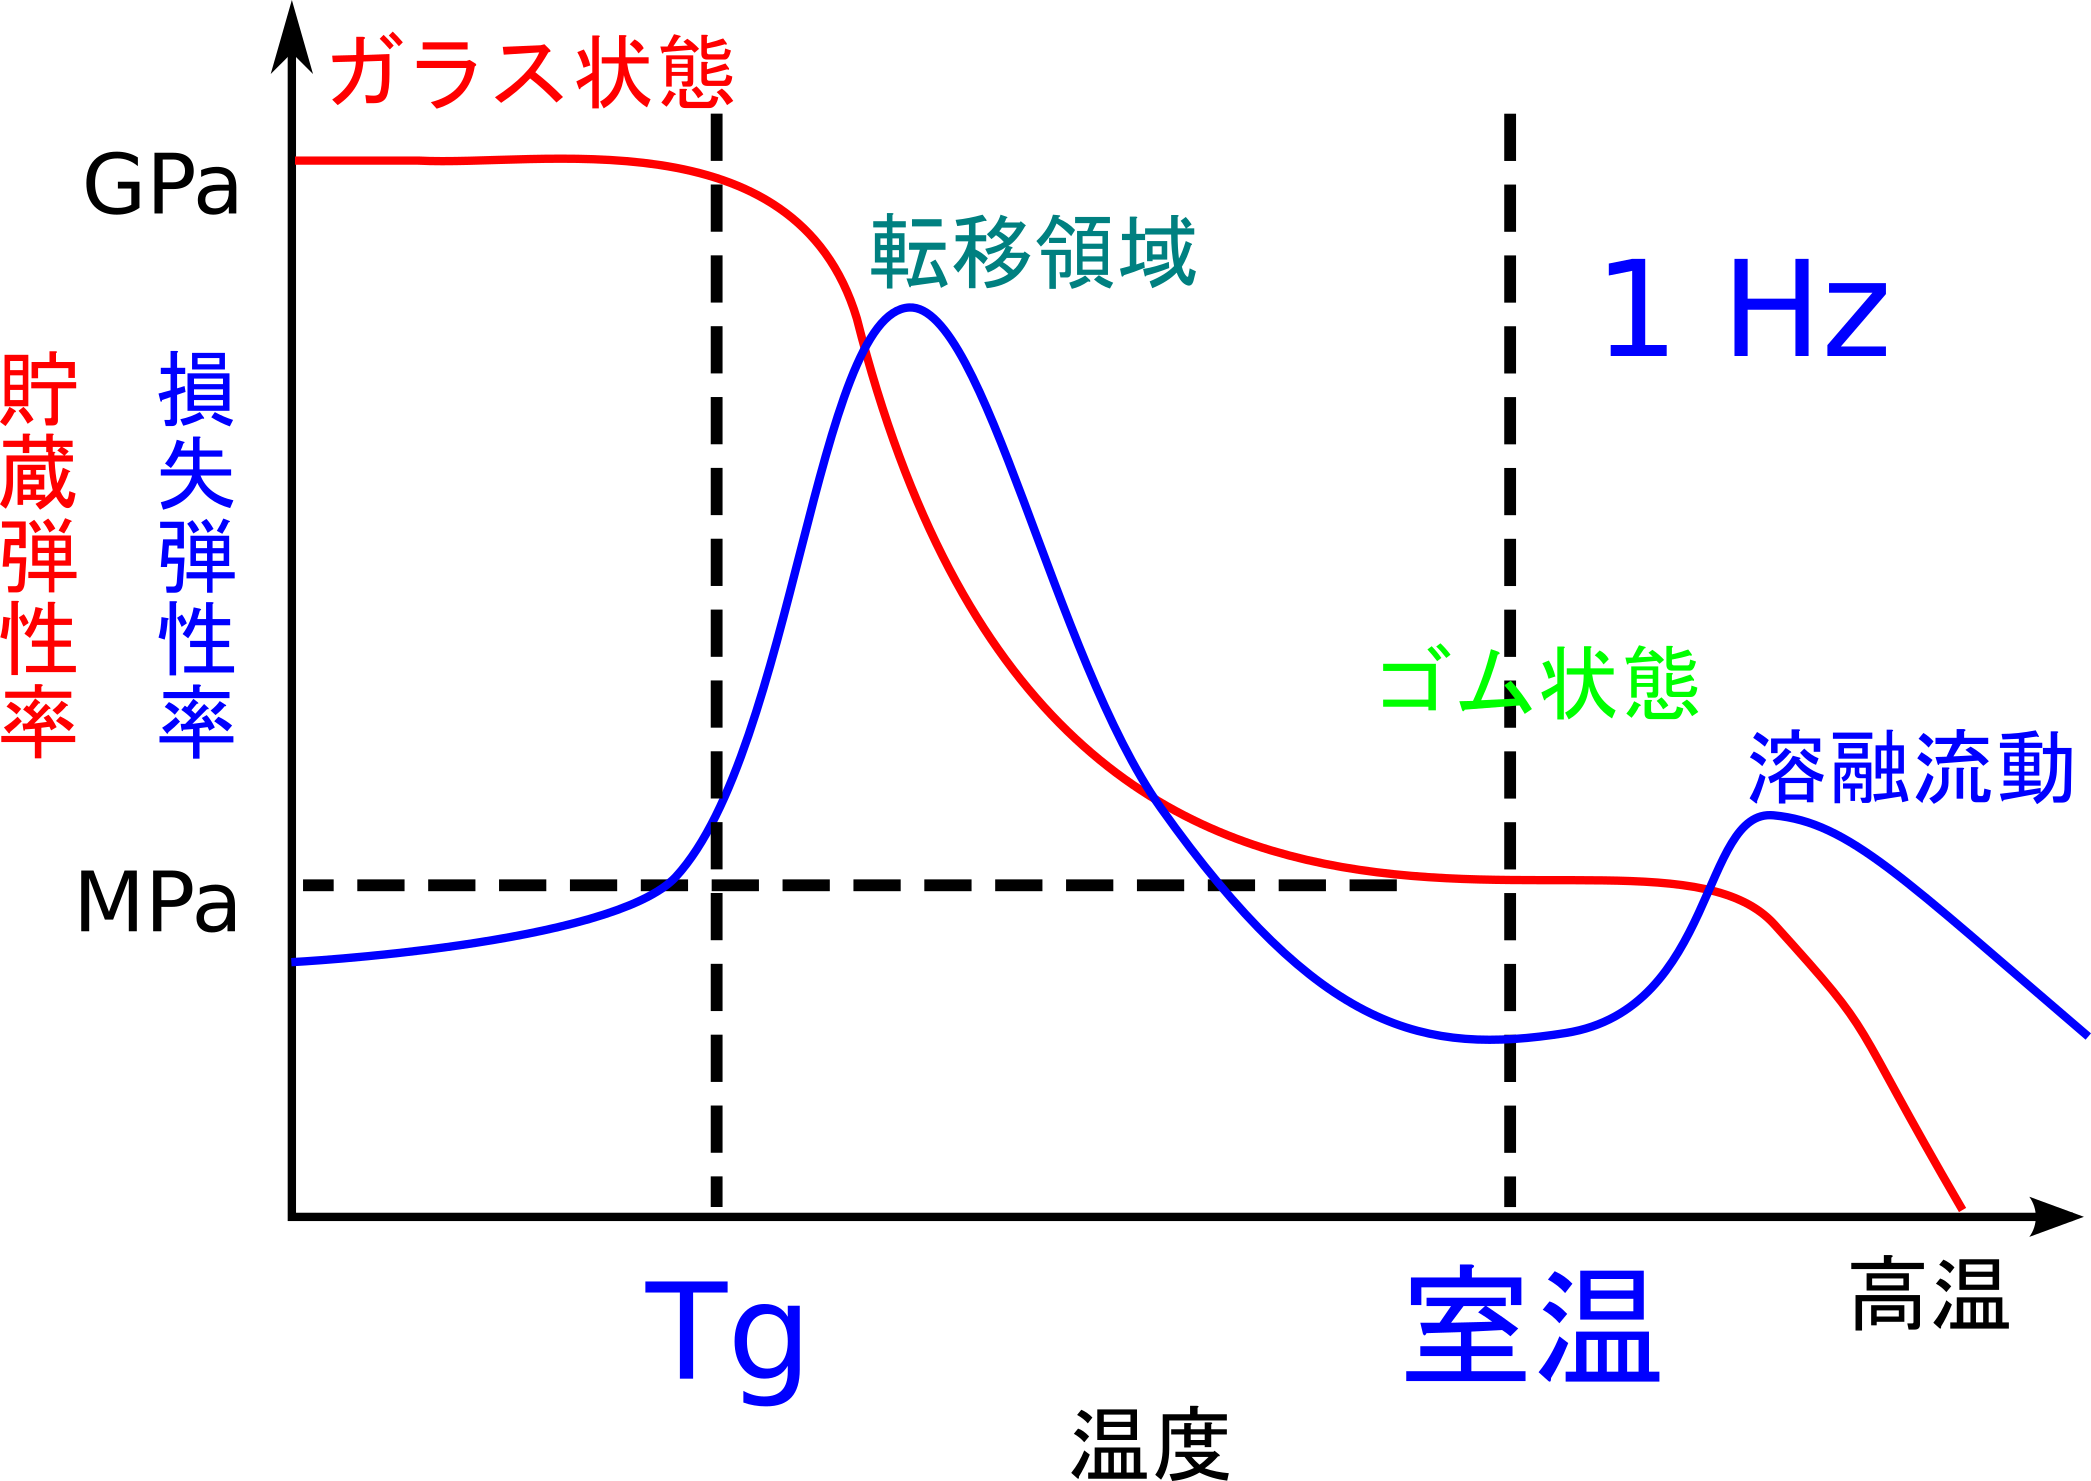
\includegraphics[width=.5\textwidth]{dynamic_ViscoElast_Temp_rubber.png}
\end{frame}

\begin{frame}
	\frametitle{ゴム系ベースポリマーがタックが低い理由}
	\begin{block}{Chang の窓で考えると}
		\begin{itemize}
			\item ラバープラトーの貯蔵弾性率が比較的に高い
			\begin{itemize}
				\item 低周波でも高周波でもあまり変化がない
			\end{itemize}
			\item ガラス転移温度が低い\\⇔転移領域に起因した損失弾性率が小さい
		\end{itemize}
	\end{block}
		\centering
			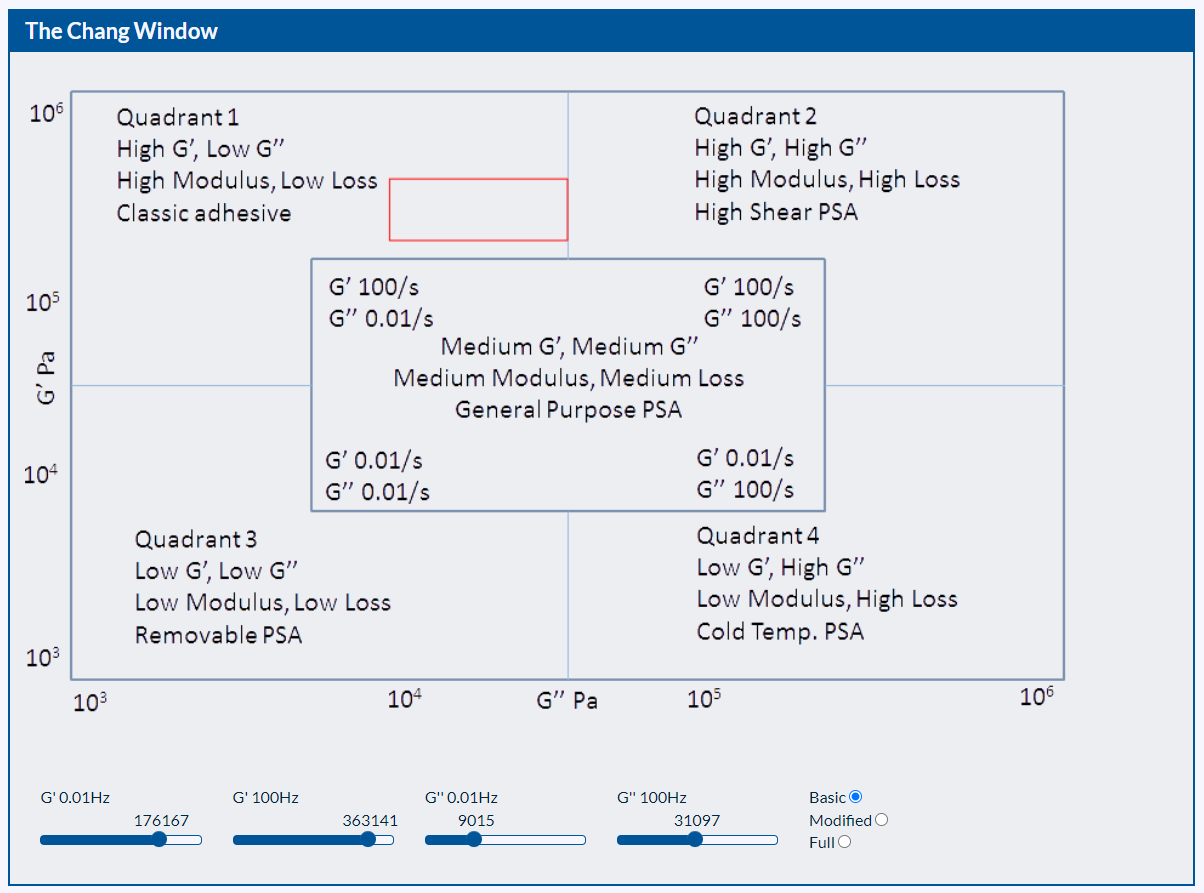
\includegraphics[width=.45\textwidth]{ChangFrequencies_rubber.png}
\end{frame}

\begin{frame}
	\frametitle{適切なタッキファイヤーの添加}

	\begin{itemize}
		\item ガラス転移温度を上昇
		\begin{itemize}
			\item エラストマーの T$_g$ = 240 K
			\item タッキファイヤーの T$_g$ = 370 K
			\item 30 \% 添加を想定
			\begin{align*}
				&\dfrac{1}{T_g} = \dfrac{0.3}{370} + \dfrac{0.7}{240} \\
				\therefore \quad &T_g \simeq 268
			\end{align*}
			\item 約30℃ガラス転移温度を上昇
			\item ガラス転移温度に起因した\alert{転移領域を室温付近}に
		\end{itemize}
		\item \alert{ガラス転移温度以上では可塑剤}として働く
		\begin{itemize}
			\item ラバープラトーの\alert{貯蔵弾性率を低下}
		\end{itemize}
	\end{itemize}
			% \centering
			% 	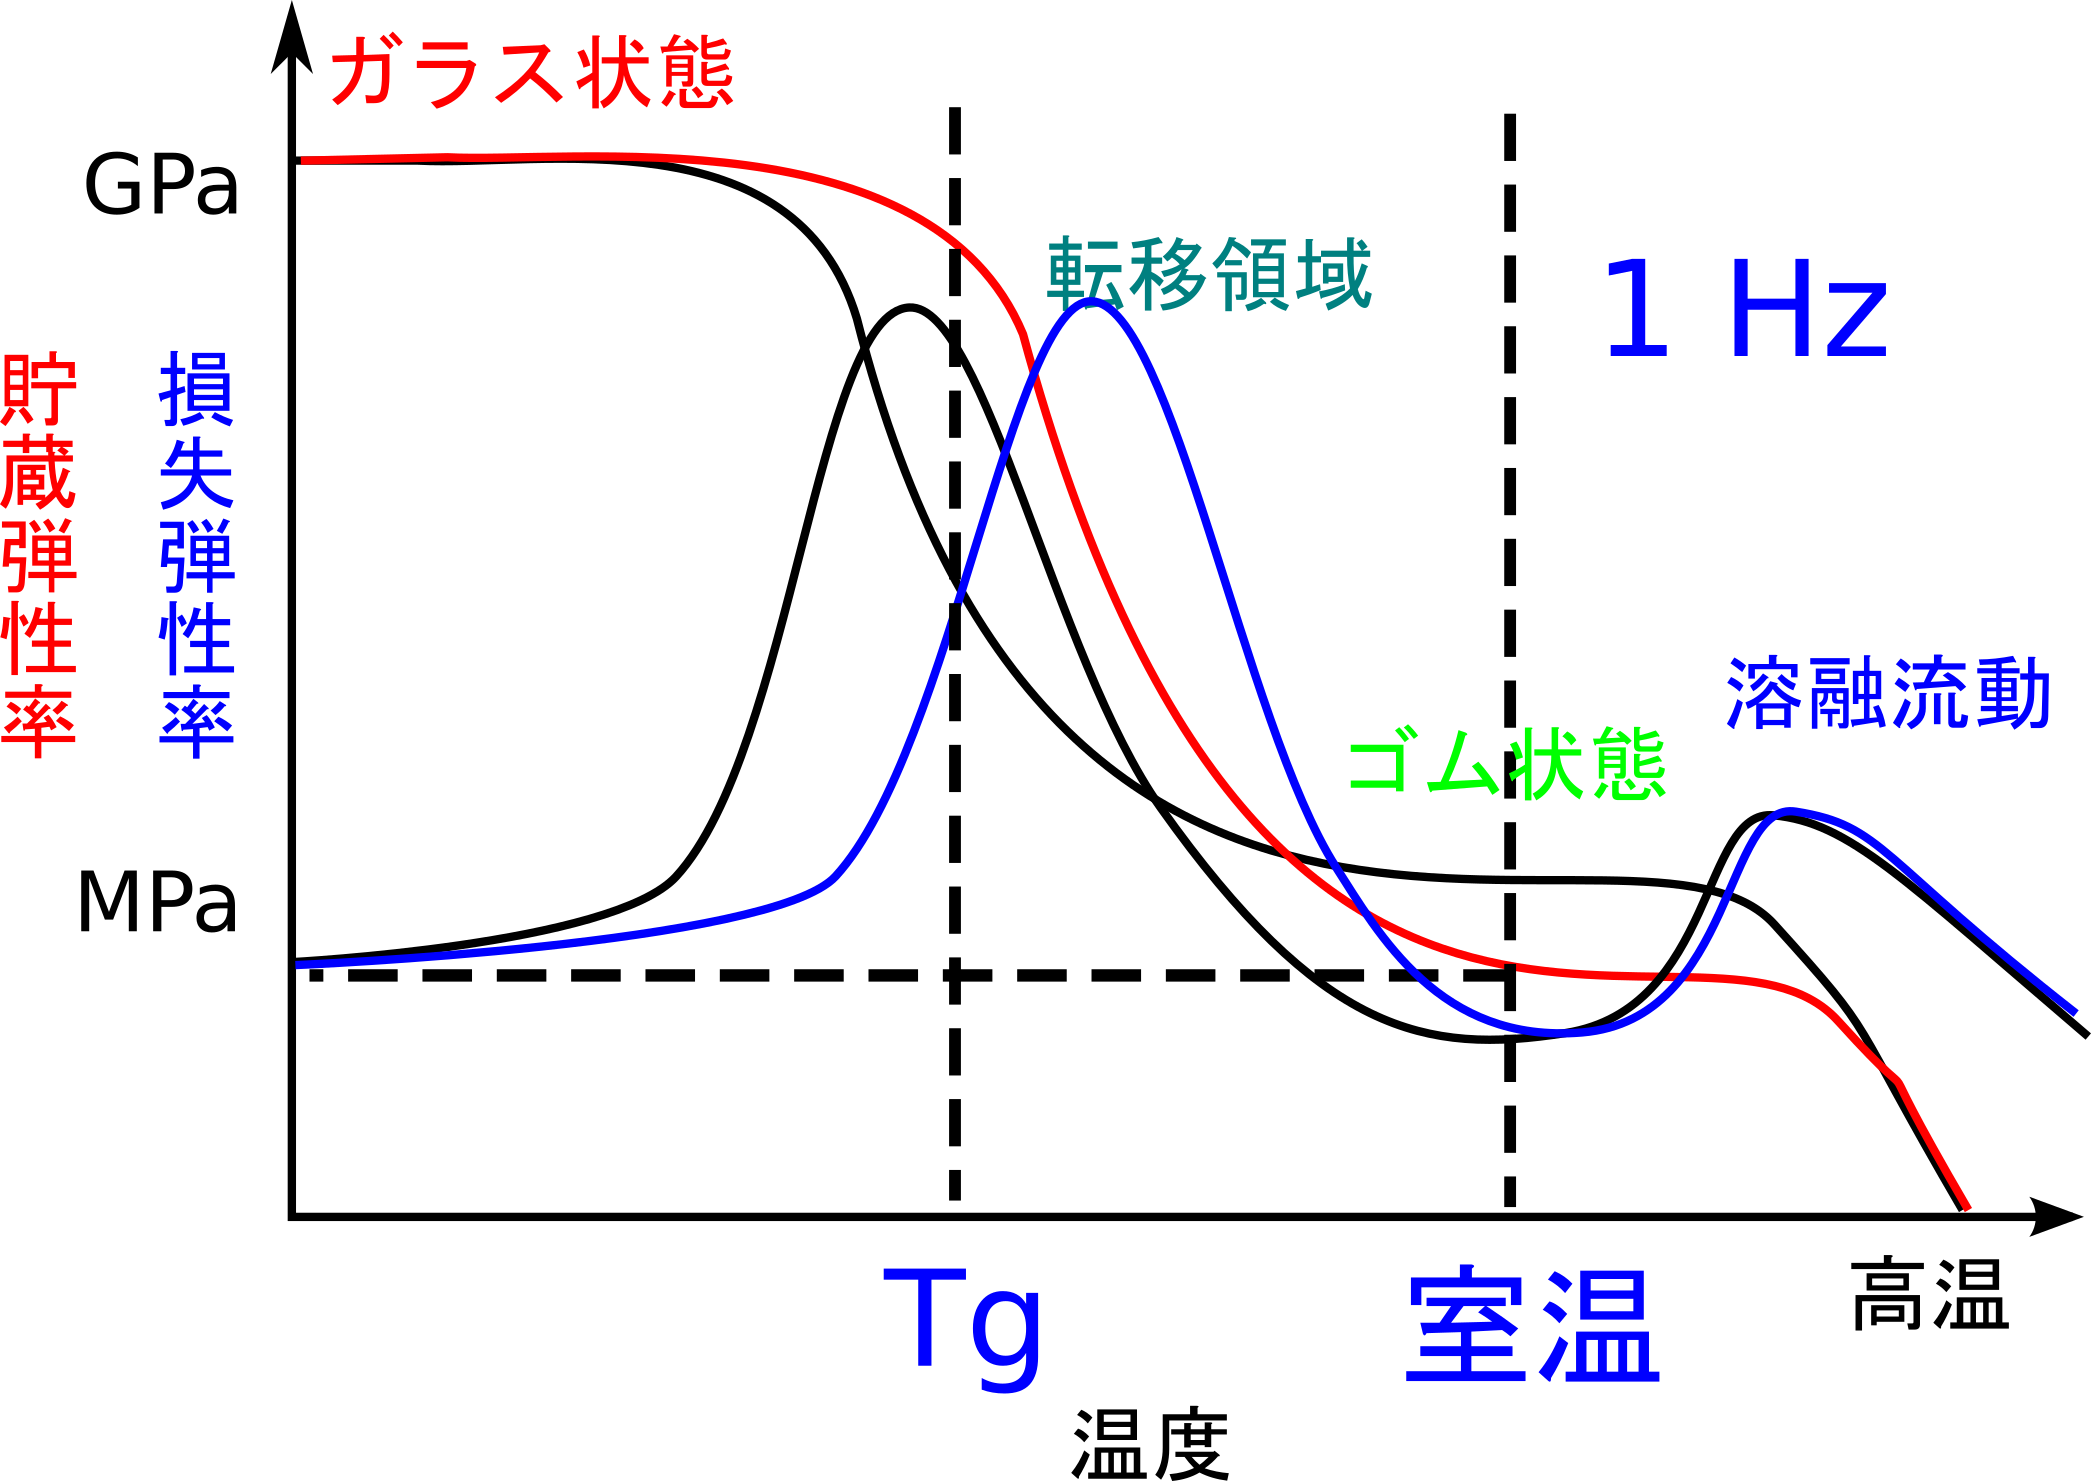
\includegraphics[width=\textwidth]{dynamic_ViscoElast_Temp_rubber_tack.png}
\end{frame}

\begin{frame}
	\frametitle{適切なタッキファイヤーの添加}
		\large{\alert{タッキファイヤー添加前後の比較}}
		\vspace{5mm}
			\centering
				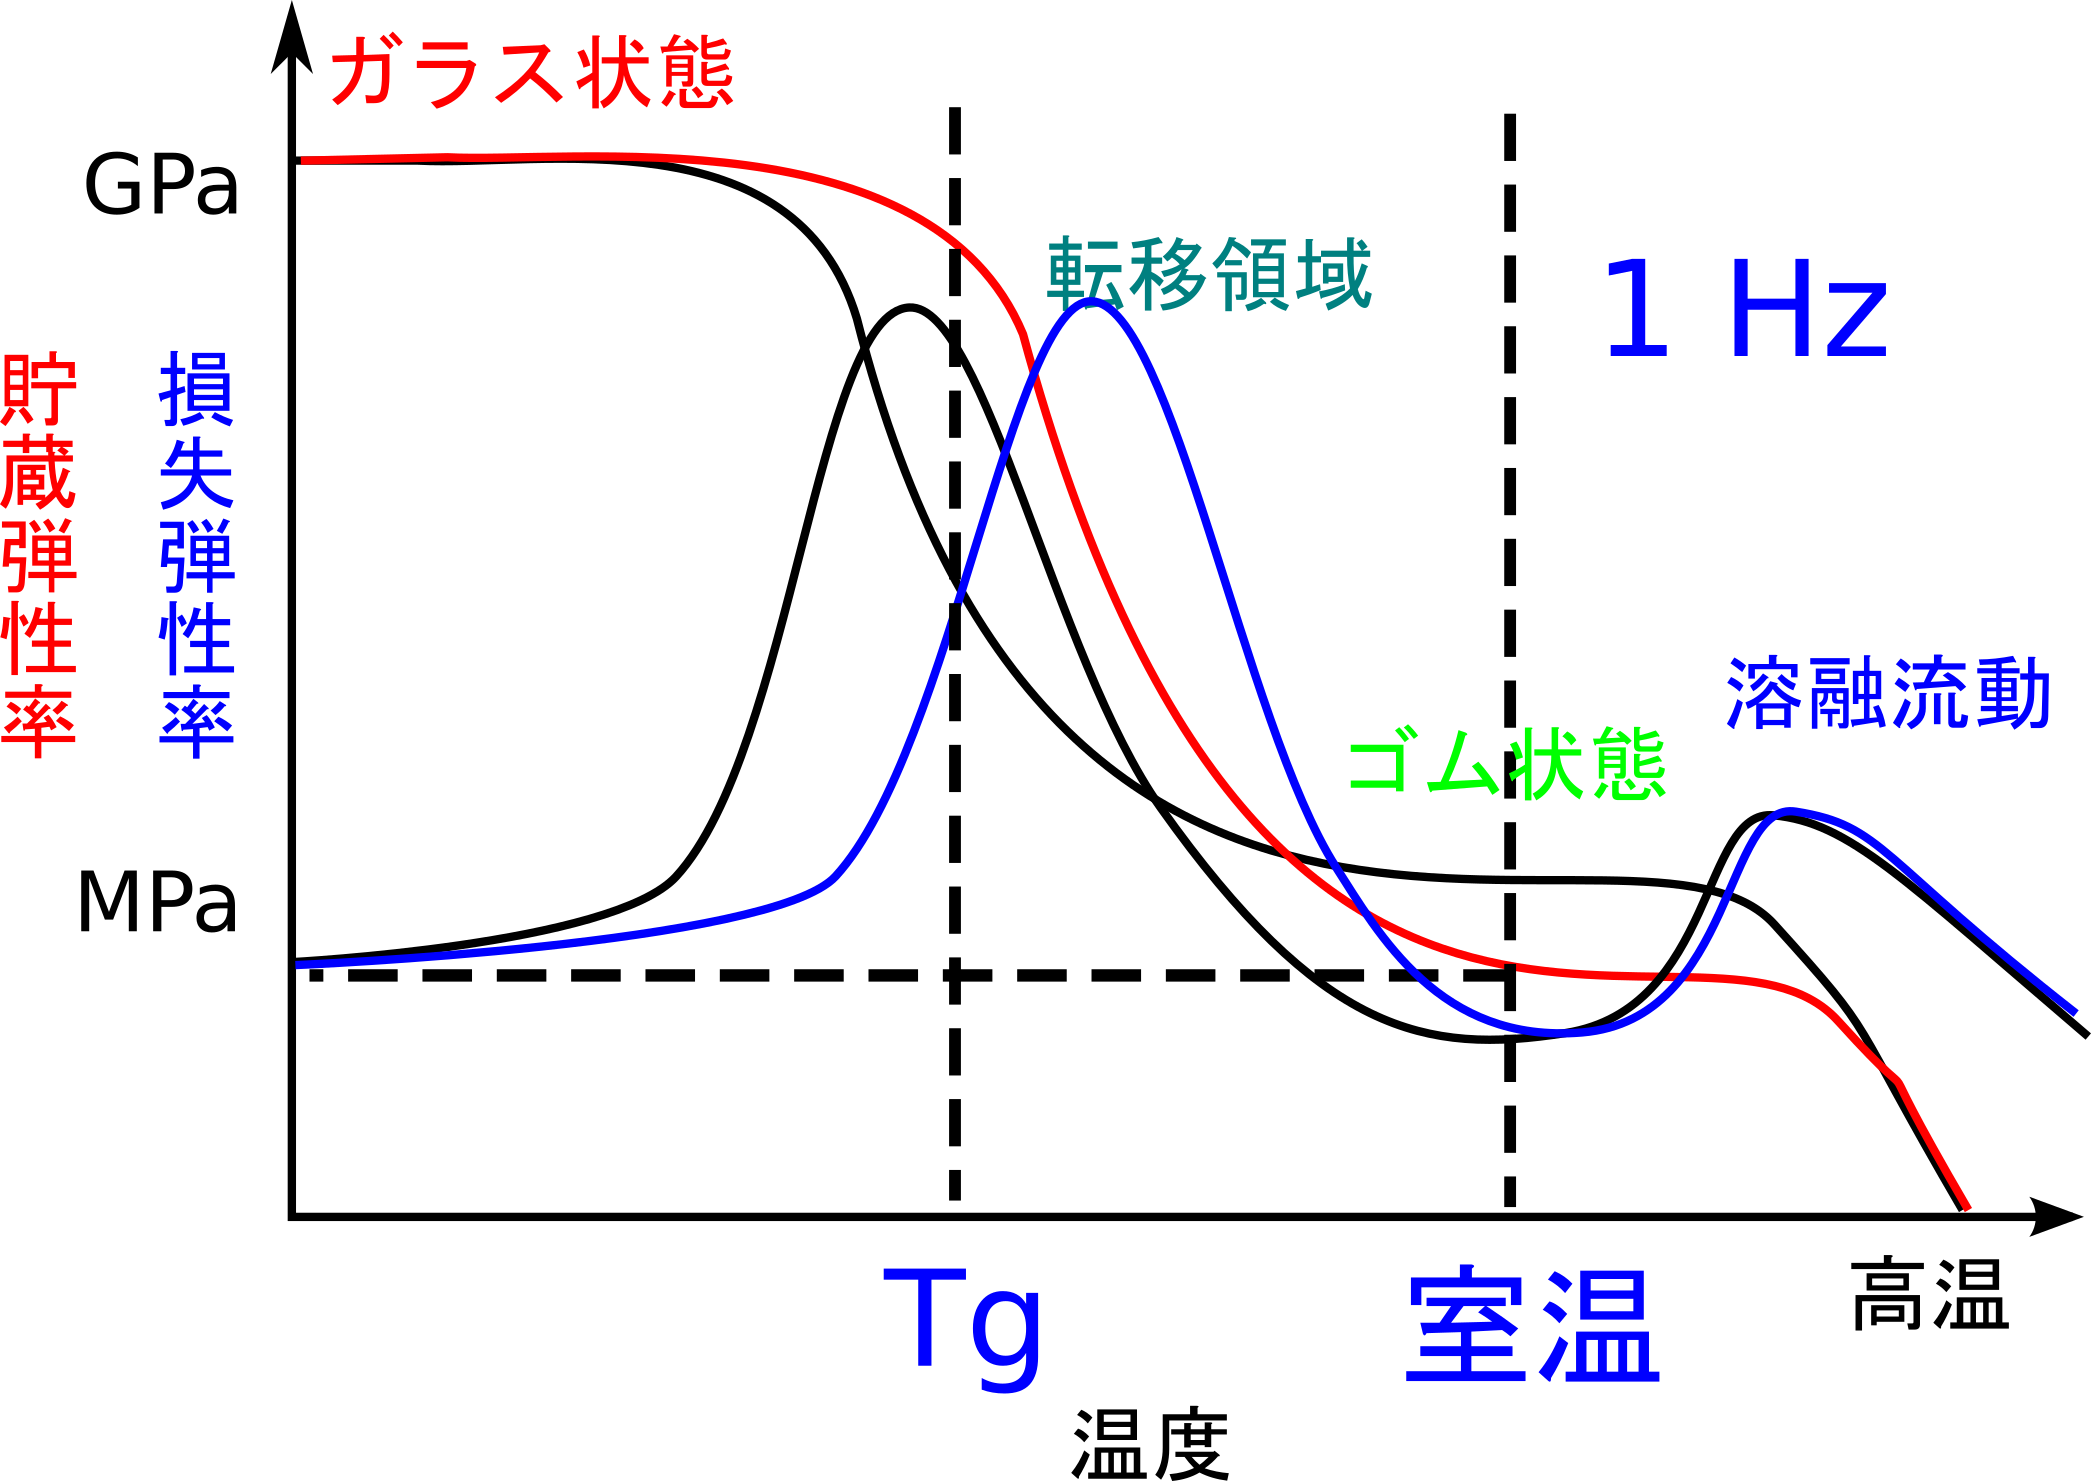
\includegraphics[width=.8\textwidth]{dynamic_ViscoElast_Temp_rubber_tack.png}
\end{frame}

\begin{frame}
	\frametitle{適切なタッキファイヤーの添加}
		\large{\alert{周波数分散と Chang の窓のイメージ}}
		\vspace{5mm}
			\centering
				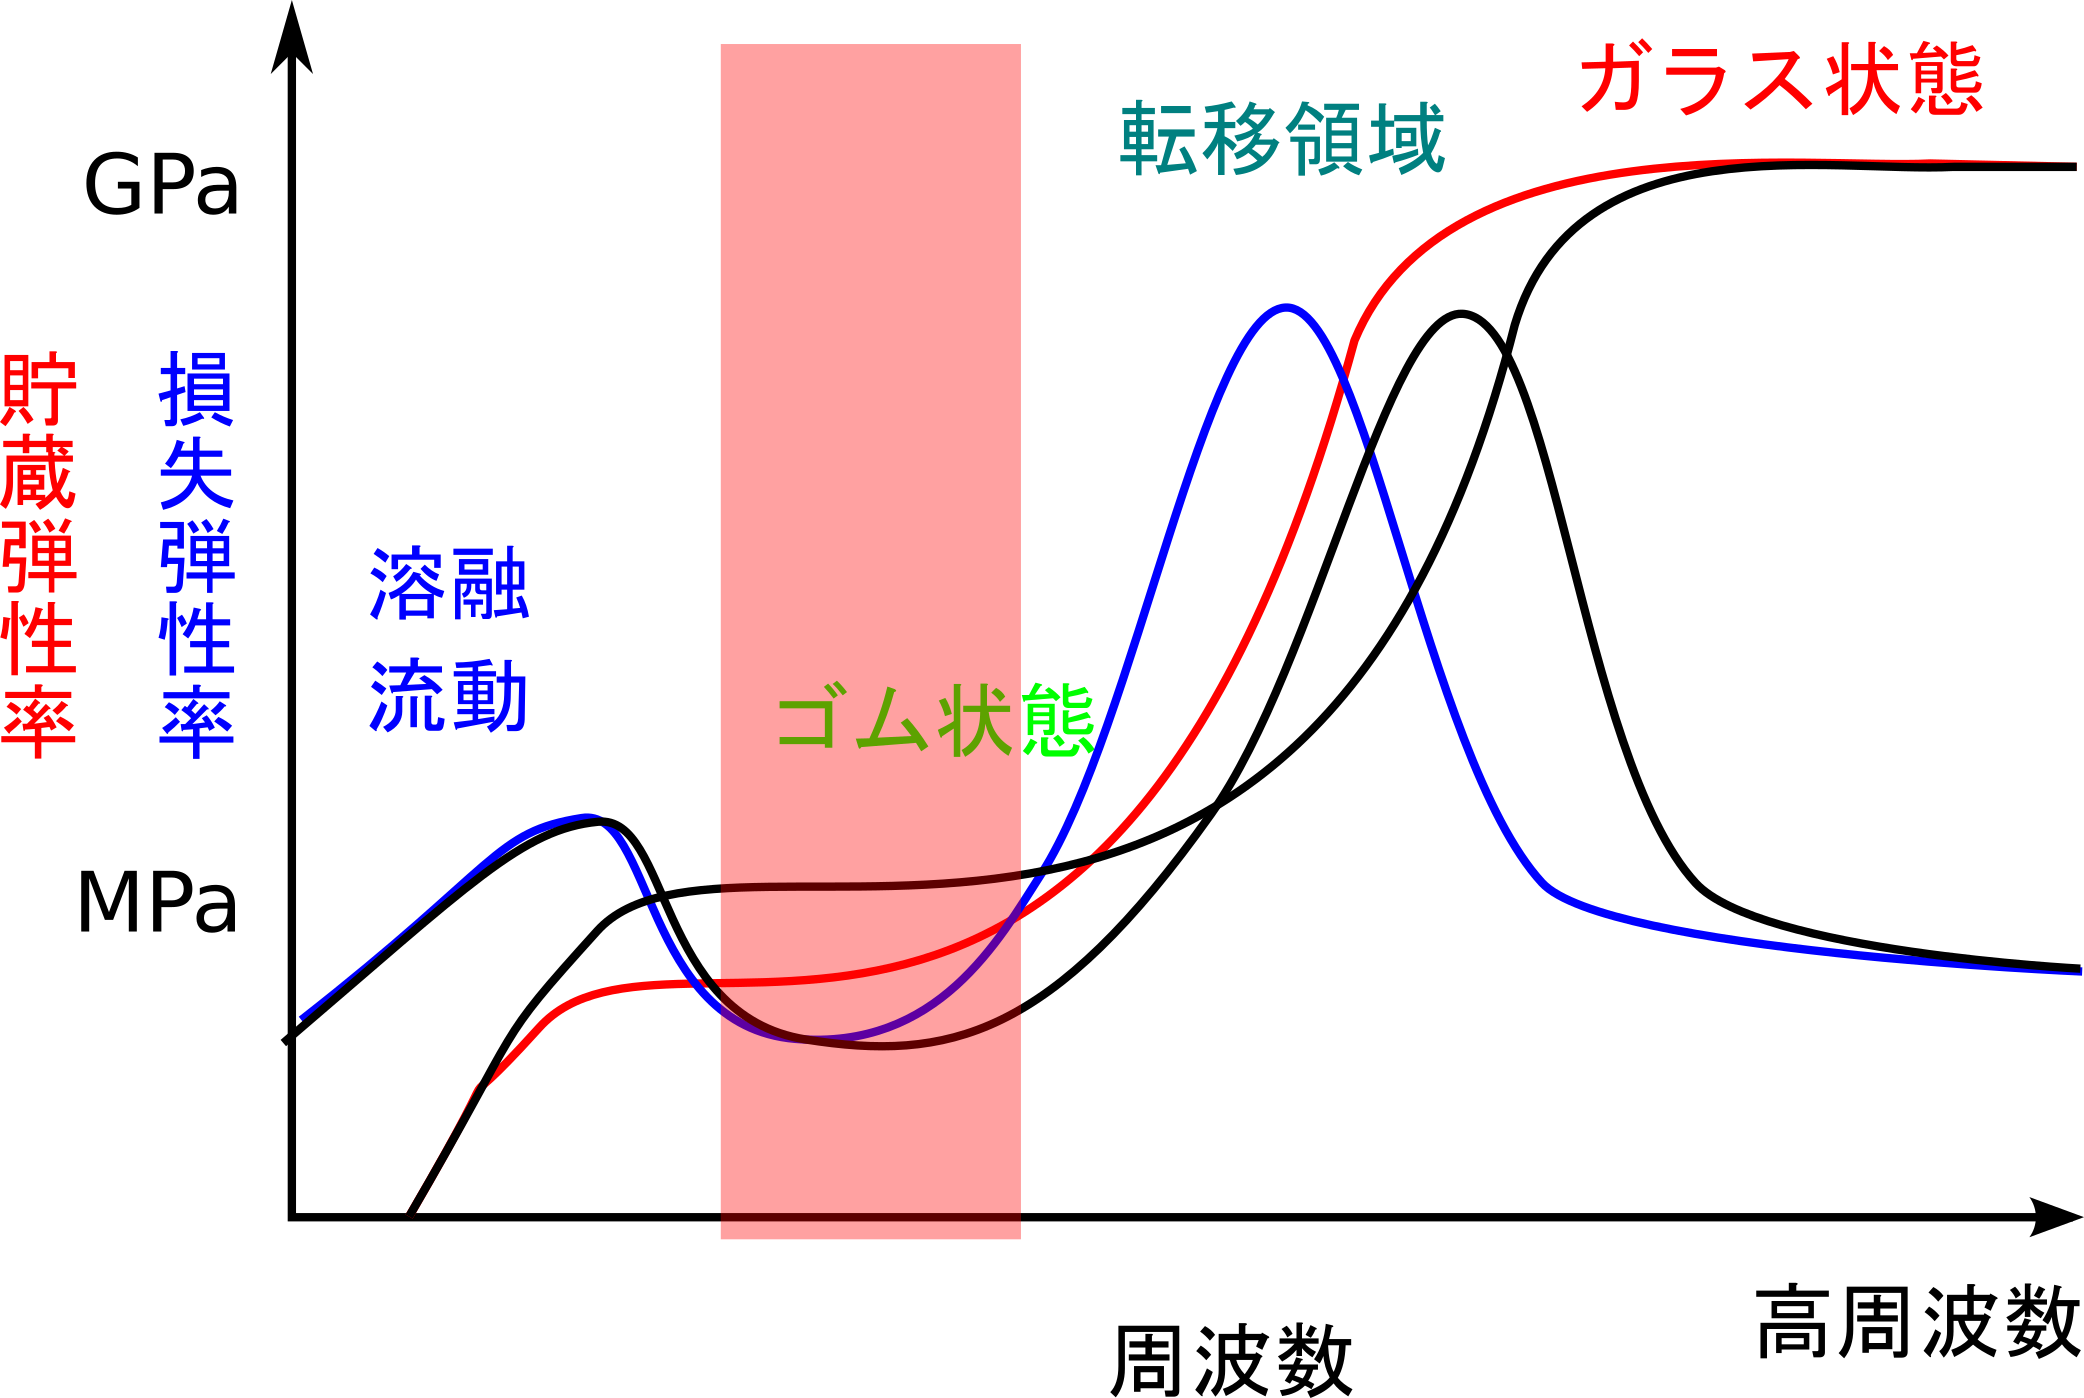
\includegraphics[width=.8\textwidth]{dynamic_ViscoElast_Freq_rubber.png}
\end{frame}


\begin{frame}
	\frametitle{適切なタッキファイヤーの添加}
		\begin{alertblock}{周波数依存の挙動をチューニング}
			\begin{itemize}
				\item 高い周波数(100/sec)
				\begin{itemize}
					\item 高い $G^{\prime \prime} \Leftrightarrow$ 高い流動性:クイックタッキネス
				\end{itemize}
				\item 低い周波数(0.01/sec)
				\begin{itemize}
					\item 低い $G^{\prime \prime} \Leftrightarrow$ 変形を抑止;保持力向上
				\end{itemize}
			\end{itemize}

			\vspace{3mm}
			\centering
				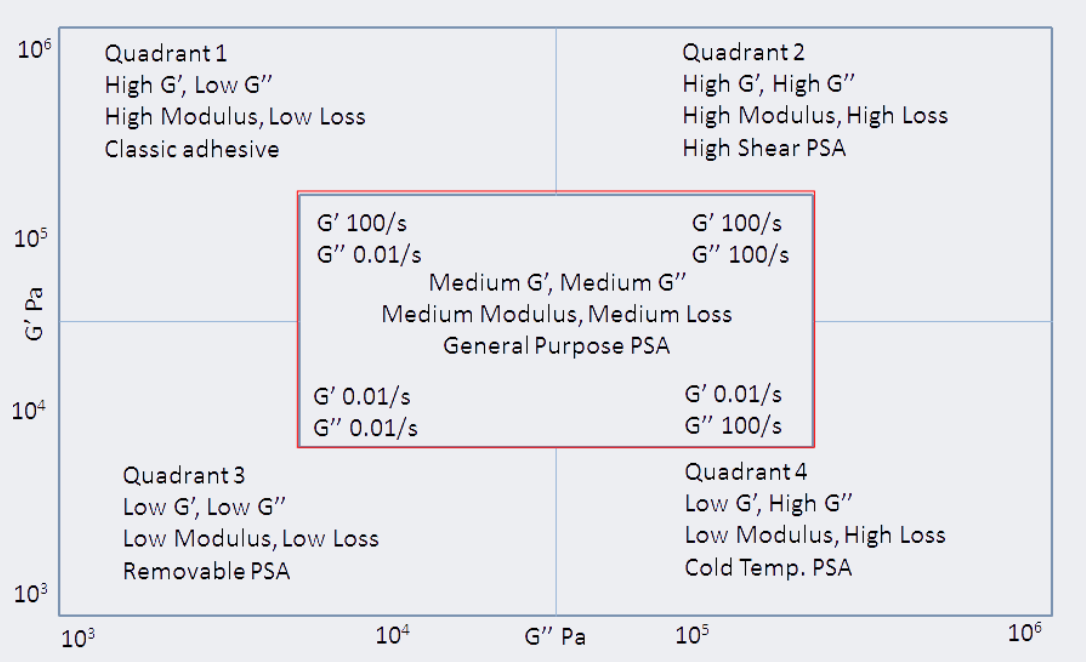
\includegraphics[width=.5\textwidth]{ChangFrequencies_2.png}
		\end{alertblock}	
\end{frame}

\subsection{アクリル系粘着剤では}
\begin{frame}
	\frametitle{アクリル系ポリマーベースの粘着剤}

	\begin{itemize}
		\item アクリル系ポリマーでは、
		\begin{itemize}
			\item 各種モノマーの共重合により\\
			⇔ガラス転移温度が調整可能
			\item 絡み合い点間分子量が大きい\\
			⇔ラバープラトーの貯蔵弾性率が比較的低い
		\end{itemize}
		\item その結果
		\begin{itemize}
			\item タッキファイヤーが必須というわけではない
			\item 各種物性調整のために利用はされる
		\end{itemize}
	\end{itemize}
\end{frame}

\begin{frame}
	\frametitle{「タッキファイヤーの添加効果」のまとめ}
        \begin{boxnote}
            \vspace{-3mm}
            \begin{itemize}
                \item タッキファイヤーの添加
                    \begin{itemize}
                        \item 種類選択で各種エラストマーとの相溶性を確保
                        \item 分子量が低いことも相溶性に有利
                    \end{itemize} 
                \item タック発現の機構
                    \begin{itemize}
                        \item ゴム状エラストマー単独では粘着特性に劣る
                        \item 適切なタッキファイヤーで特性改良が可能
                    \end{itemize} 
                \item アクリル系ポリマーベースの粘着剤
                    \begin{itemize}
                        \item ガラス転移温度、ラバープラトーの弾性率の\\調整が容易
                        \item タッキファイヤーが必須というわけではない
                    \end{itemize}
            \end{itemize}
        \end{boxnote}
\end{frame}

\end{document}